%% TITLE	Physiological Fluid Mechanics, Summary 3

%% DATE		- May 17, 2022     first release
%%          - Nov 19, 2023      update

%% AUTHOR	BINGHUAN W LI (Dept. Chemical Eng/Bio Eng, Imperial)
%%          PETER Y XIE (Dept. Mech Eng, Stanford)

%% compiled in XeLaTeX with Tex Live version 2023.

%% This work is licensed under a Creative Commons Attribution-NonCommercial 4.0 International License.

\documentclass[a4paper]{article}
\newcommand{\summaryNo}{3}
%% TITLE	Physiological Fluid Mechanics, configuration

%% DATE		- Nov 19, 2023     create

%% AUTHOR	BINGHUAN W LI (Dept. Chemical Eng/Bio Eng, Imperial)
%%          PETER Y XIE (Dept. Mech Eng, Stanford)

%% compiled in XeLaTeX with Tex Live version 2023.

%% This work is licensed under a Creative Commons Attribution-NonCommercial 4.0 International License.

\usepackage[sfdefault]{arimo}
\usepackage[left=1.5cm, right=1.5cm, top=2cm, bottom=1.5cm]{geometry}
\usepackage{amsmath, amsfonts, amssymb, cancel}
\usepackage{unicode-math}
\setmathfont
    [    Extension = .otf,
         BoldFont = XITSMath-Bold,
    ]{XITSMath-Regular}

% % \DeclareMathSizes{10}{12}{10}{9}

% \usepackage{siunitx}
\usepackage{enumitem}
\usepackage{xcolor}
    \definecolor{linkcolour}{rgb}{0,0.2,0.6}
\usepackage{hyperref}
\hypersetup{
    colorlinks,
    breaklinks,
    urlcolor=linkcolour,
    linkcolor=linkcolour,
    citecolor=black,
    pdfauthor={Li, Binghuan W},
    }
\usepackage{graphicx, float}
\usepackage{framed}
\usepackage[export]{adjustbox}

\usepackage{fancyhdr}
    \pagestyle{fancy}
    \fancyhf{}
    \lhead{\textsc{Physiological Fluid Mechanics Summary \summaryNo}}
    \rhead{page \thepage}

\usepackage{tcolorbox}

\usepackage{tikz, circuitikz}

\usepackage{multicol}
    \setlength{\columnseprule}{1pt}

\usepackage{lscape}

\usepackage{booktabs}

\usepackage{pifont}

\setlength\parindent{0pt}

\begin{document}


\section{Womersley Flow}
\paragraph{Motivation}  To study and approximate the pulsatility nature of the flow in the cardiovascular system.

\paragraph{Assumptions}
\begin{itemize}
    \item Flow in a long straight tube, with a perfect circular cross-section at radius $a$;

    \item Fluid is homogeneous, incompressible and Newtonian with viscosity $\mu$ and density $\rho$;
    
    \item Axisymmetric along the $\theta$-axis: $\displaystyle \frac{\partial}{\partial \theta}=0$; 

    \item The flow is fully developed along the $z$-axis: $\displaystyle \frac{\partial u}{\partial z}=0$; 

    \item No swirl: $u_{\phi}=0$;

    \item No velocity along the radial direction: $u_r = 0$;

    \item Neglected body force.
\end{itemize}

\paragraph{Boundary Conditions} No-slip condition on the wall, parabolic condition as Poiseuille flow.

\paragraph{Solution Procedure (at a glance)}
\begin{enumerate}[label=\underline{\textit{Step \arabic*}}]
    \item The $z$-momentum equation
    \[
        \rho \bigg(\frac{\partial u_{z}}{\partial t} + \cancelto{0}{u_{r} \frac{\partial u_{z}}{\partial r}} + \cancelto{0}{\frac{u_{\theta}}{r}\frac{\partial u_{z}}{\partial \theta}} + \cancelto{0}{u_{z}\frac{\partial u_{z}}{\partial z}} \bigg) = -\frac{\partial p}{\partial z} + \mu \bigg[ \frac{1}{r}\frac{\partial}{\partial r} \bigg(r \frac{\partial u_{z}}{\partial r}\bigg) + \cancelto{0}{\frac{1}{r^{2}} \frac{\partial^{2} u_{z}}{\partial \theta^{2}}} + \cancelto{0}{\frac{\partial^{2} u_{z}}{\partial z^{2}}} \bigg] + \cancelto{0}{\rho f_{z}}
    \]
    \[
        \Rightarrow \quad \rho \frac{\partial u_z}{\partial t} = -\frac{\partial p}{\partial z} + \mu \frac{1}{r} \frac{\partial}{\partial r} \bigg(r\frac{\partial u_z}{\partial r} \bigg).
    \]
    Assume the pressure gradient is sinusoidal: $\displaystyle \partial p / \partial z = \frac{G_0}{2}e^{i\omega t}$, and following the sinusoidal $z$-velocity: $u_z = U(r) e^{i\omega t}$:
    \[
        \bigg[ i\omega U \rho + \frac{G_0}{2} - \mu \frac{1}{r}\frac{\partial}{\partial r} \bigg(r\frac{\partial U}{\partial r}\bigg) \bigg] e^{i\omega t} = 0
        \quad \xrightarrow[]{\text{2\textsuperscript{nd}-order ODE}} \quad
        \frac{\partial^2 U}{\partial r^2} + \frac{1}{r} \frac{\partial U}{\partial r} - \frac{i\omega \rho}{\mu} U = \frac{G_0}{2\mu}.
    \]

    \item The full solution of $U(r)$ involves a complementary function, which is formulated with the Bessel function of the 1\textsuperscript{st} kind at 0\textsuperscript{th} order, $J_0$; also the particular integral, $U_{pi} = -G_0 / 2i\omega \rho$:
    \[\
        U(r) = \frac{iG_{0}}{2\omega \rho}\bigg[ 1- \frac{J_{0}(i^{3/2}\alpha \frac{r}{a})}{J_{0}(i^{3/2}\alpha)} \bigg],
    \]
    where
    \[
        J_0(s) = \sum_{k=0}^{+\infty} \frac{(-1)^k}{k!k!}\bigg(\frac{s}{2}\bigg)^{2k},
    \]
    and $\alpha$ denotes the non-dimensional \textbf{Wormersley number}: $\displaystyle \alpha = a \sqrt{\frac{\omega}{\nu}}$ (the ratio between unsteady inertia force to viscous force).
    
    \item To recover $u_z$ from $U(r)$:
    \[
        u_{z}(r,t) = \frac{i}{\omega \rho} \frac{\partial p}{\partial z} \bigg[ 1- \frac{J_{0}(i^{3/2}\alpha \frac{r}{a})}{J_{0}(i^{3/2}\alpha)} \bigg] e^{i\omega t} = \frac{iG_{0}}{2\omega \rho}\bigg[ 1- \frac{J_{0}(i^{3/2}\alpha \frac{r}{a})}{J_{0}(i^{3/2}\alpha)} \bigg] 
    \]
    Physically, we only consider the real part of the above solution in the complex domain.
\end{enumerate}

\paragraph{Extended Properties}
\begin{enumerate}
    \item  Wall shear stress: 
    \[
        \tau_{rz} = \mu \frac{\partial u_{z}}{\partial r} = \mathrm{Re}\bigg\{ -\frac{a}{i^{3/2}\alpha} \bigg( \frac{J_{1}(i^{3/2}\alpha)}{J_{0}(i^{3/2}\alpha)} \bigg) \frac{\partial p}{\partial z} \bigg\}, \quad 
        \text{where} \ \ J_n = \sum_{k=0}^{+\infty} \frac{(-1)^k}{k!(k+n)!} \bigg(\frac{s}{2}\bigg)^{2k+n}.
    \]

    \item Volume flow rate: 
    \[
        Q(t) = \int_{0}^{a} 2\pi r u_{z} \mathrm{d}r = \mathrm{Re}\bigg\{ -\frac{\pi a^{4}}{i \mu \alpha^{2}} \bigg( 1 - \frac{2J_{1}(i^{3/2}\alpha)}{\alpha i^{3/2} J_{0}(i^{3/2}\alpha)} \bigg) \frac{\partial p}{\partial z} \bigg\}.
    \]
\end{enumerate}

\begin{figure}[H]
    \centering
    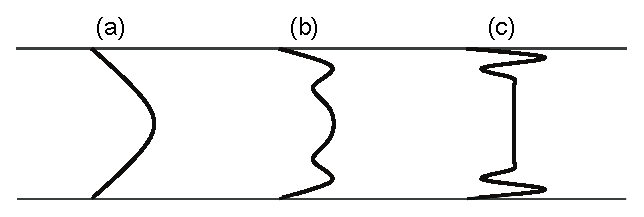
\includegraphics[width=.4\textwidth]{img/wo_plot.eps}
    \caption{Womersley flow profiles. (a) Low $\alpha$ (viscous dominants), (b) intermediate $\alpha$, (c) high $\alpha$ (inertia dominates).}
\end{figure}

%% 
\section{Pipe Flow}

\subsection{Energy Equation}
\begin{itemize}
    \item The \textbf{pipe flow energy equation} (note the difference from Bernoulli's equation) states,
    \[
        \frac{p_1}{\rho g} + \frac{1}{2g}u_1^2 + z_1 = \frac{p_2}{\rho g} + \frac{1}{2g}u_2^2 + z_2 + {\color{red} h_f}
    \]
    where $\displaystyle h_{f} = f\frac{L}{D}\frac{V^{2}}{2g}$ denotes the \textbf{major head loss}, which is the energy loss due to fluid friction, , where $f$ is the Darcy friction factor. 
    
    \item For the flow in a circular pipe, if the flow is laminar (essentially, Poiseuille flow), $f = 64/Re$; Otherwise, one needs to consult the Moody chart, where the friction factor is related to the Reynolds number and the relative wall roughness of the pipe, $f(Re, \frac{\varepsilon}{d})$.
    
    \item The presence of $h_f$ leads to the pressure drop: $\Delta p = h_f \rho g$.
\end{itemize}

\subsection{Laminar and Turbulence Flow}
\begin{itemize}
    \item The Reynolds number, $Re$, measures the ratio of the momentum force to the viscus force,
    \[ 
        Re = \frac{\rho VD}{\mu} = \frac{VD}{\nu}
        = \begin{cases}
            < 2000, & \text{laminar} \\
            2000 - 3000, & \text{transient} \\
            > 3000, & \text{turbulence}
        \end{cases}.
    \]

    \item Reynolds averaging: characterize turbulent flow using statistical methods.
    \begin{center}
        \begin{tabular}{c c}
        \toprule
        average velocity    &   velocity fluctuation\\
        \midrule
        $\Bar{u} = \frac{1}{T} \int_{0}^{T} u \mathrm{d}t$     & $u' = u - \Bar{u}$\\
        \bottomrule
        \end{tabular}
    \end{center}
    Hence, the $x$-momentum equation becomes
    \[
        \rho \frac{D\Bar{u}}{Dt} = -\frac{\partial \Bar{u}}{\partial x} + \frac{\partial}{\partial x} \bigg(\mu \frac{\partial\Bar{u}}{\partial x} - \rho \overline{u'u'}\bigg) + \frac{\partial}{\partial y} \bigg(\mu \frac{\partial\Bar{u}}{\partial y} - \rho \overline{u'v'}\bigg) + \frac{\partial}{\partial z} \bigg(\mu \frac{\partial\Bar{u}}{\partial z} - \rho \overline{u'w'}\bigg) + \rho g.
    \]
\end{itemize}

\begin{landscape}
\begin{figure}
    \centering
    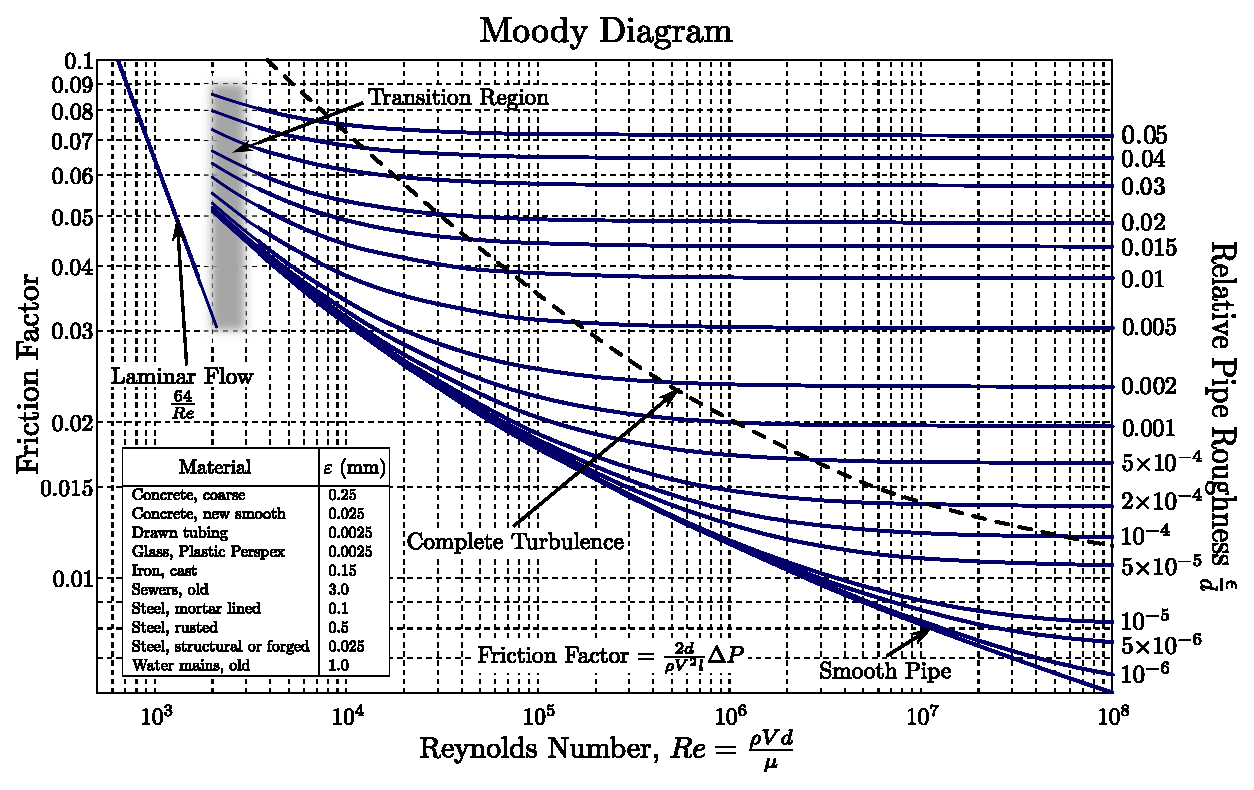
\includegraphics[scale=.8]{img/Moody_EN.eps}
    \caption{Moody's chart. Adopted from \href{https://en.m.wikipedia.org/wiki/File:Moody_EN.svg}{Wikipedia}}
    \label{fig:moody}
\end{figure}

\begin{figure}[H]
    \centering
    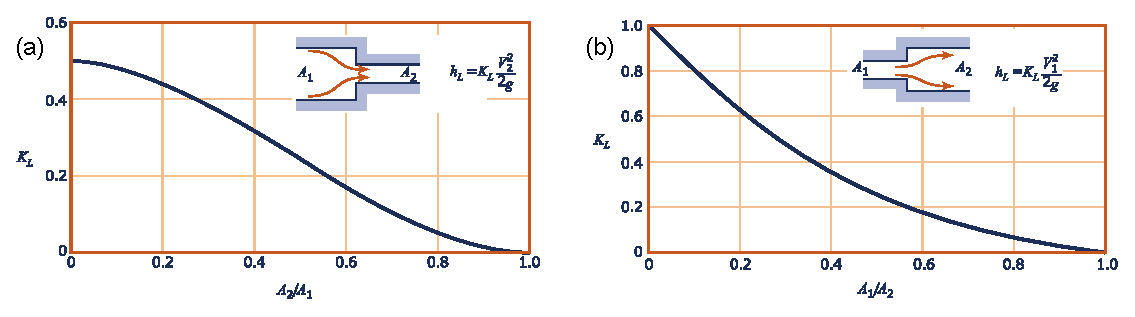
\includegraphics{img/contraction_expansion_loss.eps}
    \caption{Loss coefficient for a sudden (a) contraction, (b) expansion. Adopted from Munson \textit{et al.}, Fundamental of Fluid Mechanics, 7\textsuperscript{th} Ed.}
    \label{fig:contraction-expansion-losses}
\end{figure}
\end{landscape}


\section{Lumped Parameter Modelling}
\paragraph{Resistance, Compliance, and Intertance}
\begin{center}
    \begin{tabular}{ccc}
    \toprule
        Resistance & Compliance & Inertance  \\ [.2em]
    \midrule
        $Q = \Delta P / R$ & $\displaystyle Q = C \frac{\partial p}{\partial t}$ & $\displaystyle p = L \frac{\partial Q}{\partial t}$ \\ [.2em]
    \bottomrule
    \end{tabular}
\end{center}
\begin{itemize}
    \item Resistance: analogous to the electrical resistance - dissipation of energy.
    \item Compliance: This models the expansion of cardiovascular chambers under pressure, allowing it to store more fluid.
    \item Inertance: When the fluid momentum is substantial, when pressure is reversed on forward-flowing fluid, the fluid will not suddenly reverse its direction, but decelerate over a transient.
\end{itemize}


\paragraph{Contraction and Expansion Loss}

\[
    \Delta P = \rho g h_{f}  \quad \Rightarrow \quad R = \frac{\Delta P}{Q} = \frac{\rho g h_{f} \cdot V}{A} = \frac{\rho g K_L V}{2gA}
\]
where the value of $K_L$ can be found in \autoref{fig:contraction-expansion-losses}. Note that \autoref{fig:contraction-expansion-losses} only applies for the turbulence flow $\Rightarrow$ calculate $Re$ before applying it!

\paragraph{Solving a Lumped Parameter Network} Consider the example lumped parameter network. \\

\begin{minipage}{0.5\textwidth}
    \begin{center}
    \begin{circuitikz}
    \draw (0,0)node[label={$P_1$}]{} to [resistor, R=$R_1$, i_=$Q_1$, o-o] (3, 0)node[label={$P_2$}]{} to [resistor, R=$R_1$, i_=$Q_2$, o-o] (6,0)node[label={$P_3$}]{};
    \draw (3,0) to [capacitor, C=$C$, i_=$Q_3$, o-] (3, -2)node[ground]{} node [left=3em, below=.5em] {$P_g=0$};
    \end{circuitikz}
\end{center}

\end{minipage}
\hfill
\begin{minipage}{0.5\textwidth}
... which yields a linear system with 4 unknowns ($P_2$, $Q_1$, $Q_2$, $Q_3$) and 4 simultaneous equations:
\begin{equation}
    P_2 - P_1 = R_1 Q_1,
\end{equation}
\begin{equation}
    P_3 - P_2 = R_2 Q_2,
\end{equation}
\begin{equation}
    Q_3 = C (P_2^{(t)} - P_2^{(t-1)})/\Delta t,
\end{equation}
\begin{equation}
    Q_1 = Q_2 + Q_3.
\end{equation}
\end{minipage}

The above linear system can be re-arranged into the matrix system, $\mathbf{A}\mathbf{x} = \mathbf{b}$,
\[
    \begin{bmatrix}
        1 & -R_1 & 0 & 0 \\
        -1 & 0 & -R_2 & 0 \\
        -1 & 0 & 0 & \frac{\Delta t}{C} \\
        0 & -1 & -1 & -1\\
    \end{bmatrix}
    \begin{bmatrix}
        P_2 \\
        Q_1 \\
        Q_2 \\
        Q_3\\
    \end{bmatrix}
    =
    \begin{bmatrix}
        P_1 \\
        -P_3 \\
        -P_2^{(t-1)} \\
        0
    \end{bmatrix},
\]
and can be easily solved by inverting the coefficient matrix: $\mathbf{x} = \mathbf{A}^{-1}\mathbf{b}$.

\vfill
{\small \color{gray}Drafted by B. Li, \today}
%% TITLE	Physiological Fluid Mechanics, last page

%% DATE		- Nov 19, 2023     create

%% AUTHOR	BINGHUAN W LI (Dept. Chemical Eng/Bio Eng, Imperial)
%%          PETER Y XIE (Dept. Mech Eng, Stanford)

%% compiled in XeLaTeX with Tex Live version 2023.

%% This work is licensed under a Creative Commons Attribution-NonCommercial 4.0 International License.

\newpage
\thispagestyle{empty}
\newgeometry{margin=1.8cm}

\mbox{}
\vfill    
\begin{figure}[H]
    \includegraphics[right]{img/by-nc.eps}
\end{figure}
\textit{This work is licensed under a Creative Commons Attribution-NonCommercial 4.0 International License.}

\end{document}